\section{Delegate Ant MAS Approach}
\label{sec:dmas_algorithm}

\npar There are many possible ways of using a \textit{Delegate Ant MAS (DMAS)}
to solve the \textit{Pickup and Dellivery Problem (PDP)}. This section will
outline a solution that defines two agents:

These 

In real life situations will 


\begin{figure}[!h]
        \vspace{0.5pt}
        \begin{center}
       			\setlength\fboxsep{0.5pt}
				\setlength\fboxrule{0.5pt}
                \fbox{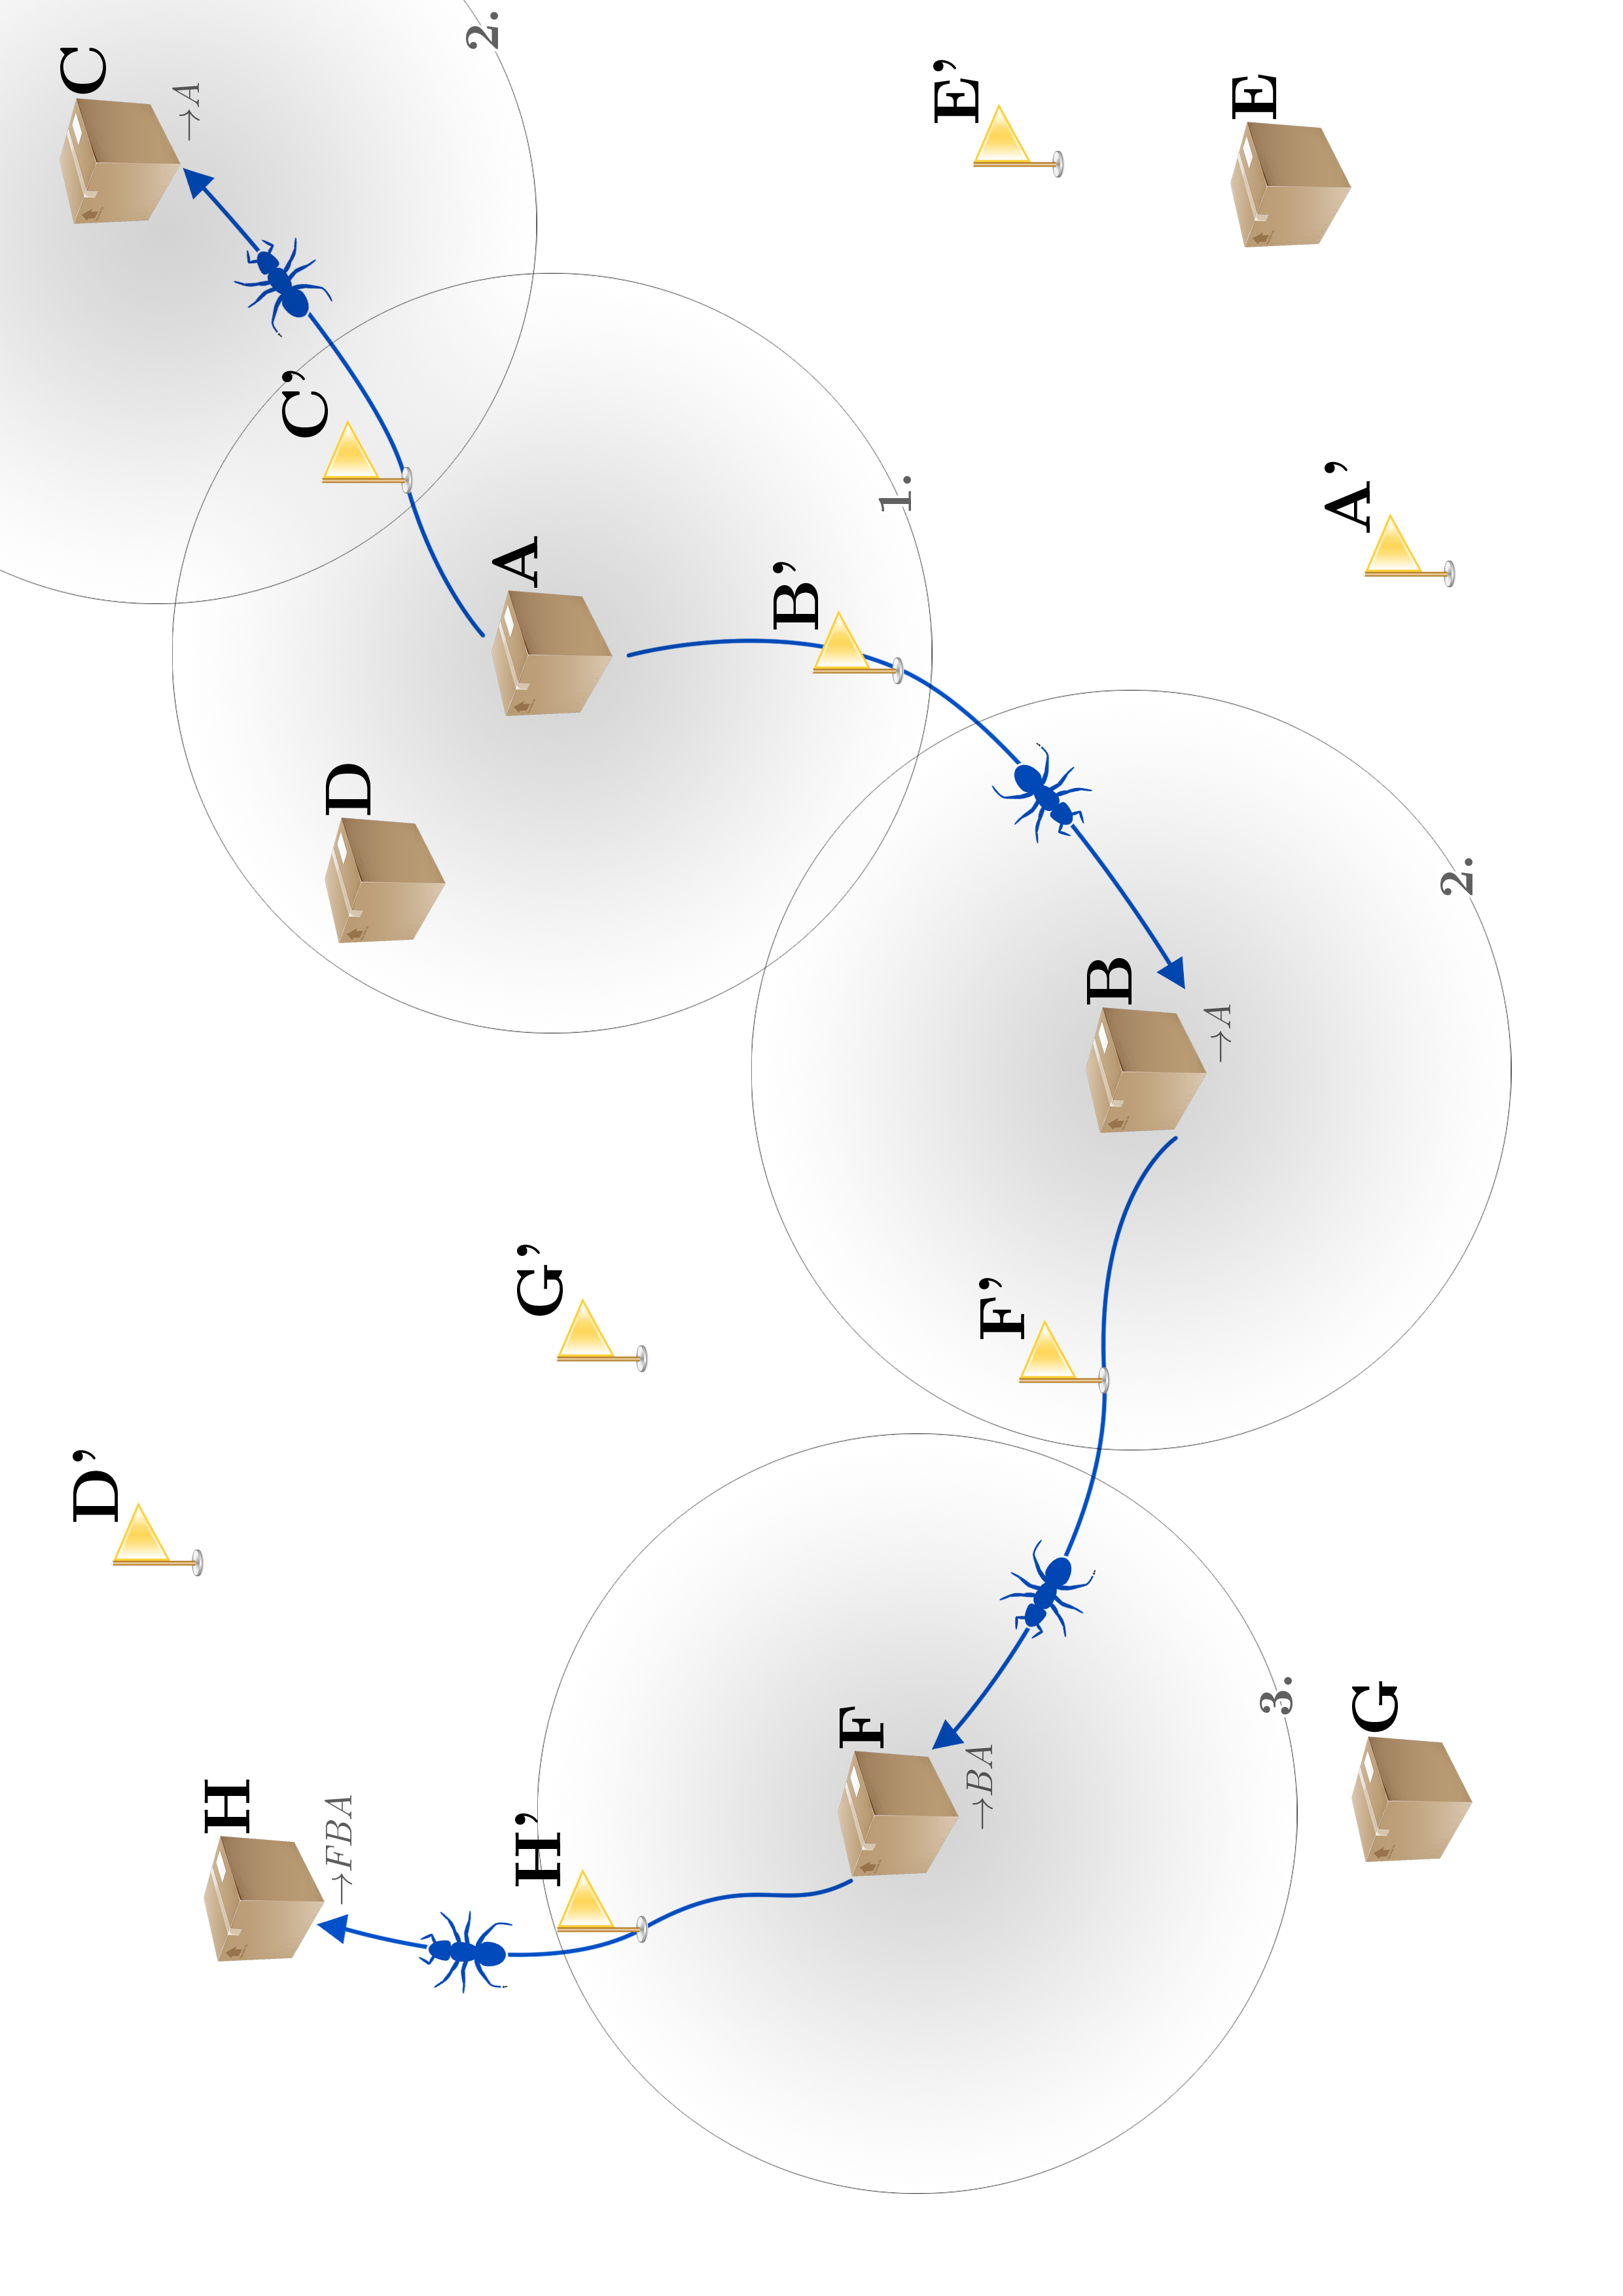
\includegraphics[width =
                0.9\textwidth]{./figs/feasibility.png}}
		\end{center}
		\caption{Feasibility Ants (example scenario 1)}
		\label{Fig:Radios}
        \vspace{0.5pt}
\end{figure}

\begin{figure}[!h]
        \vspace{0.5pt}
        \begin{center}
       			\setlength\fboxsep{0.5pt}
				\setlength\fboxrule{0.5pt}
                \fbox{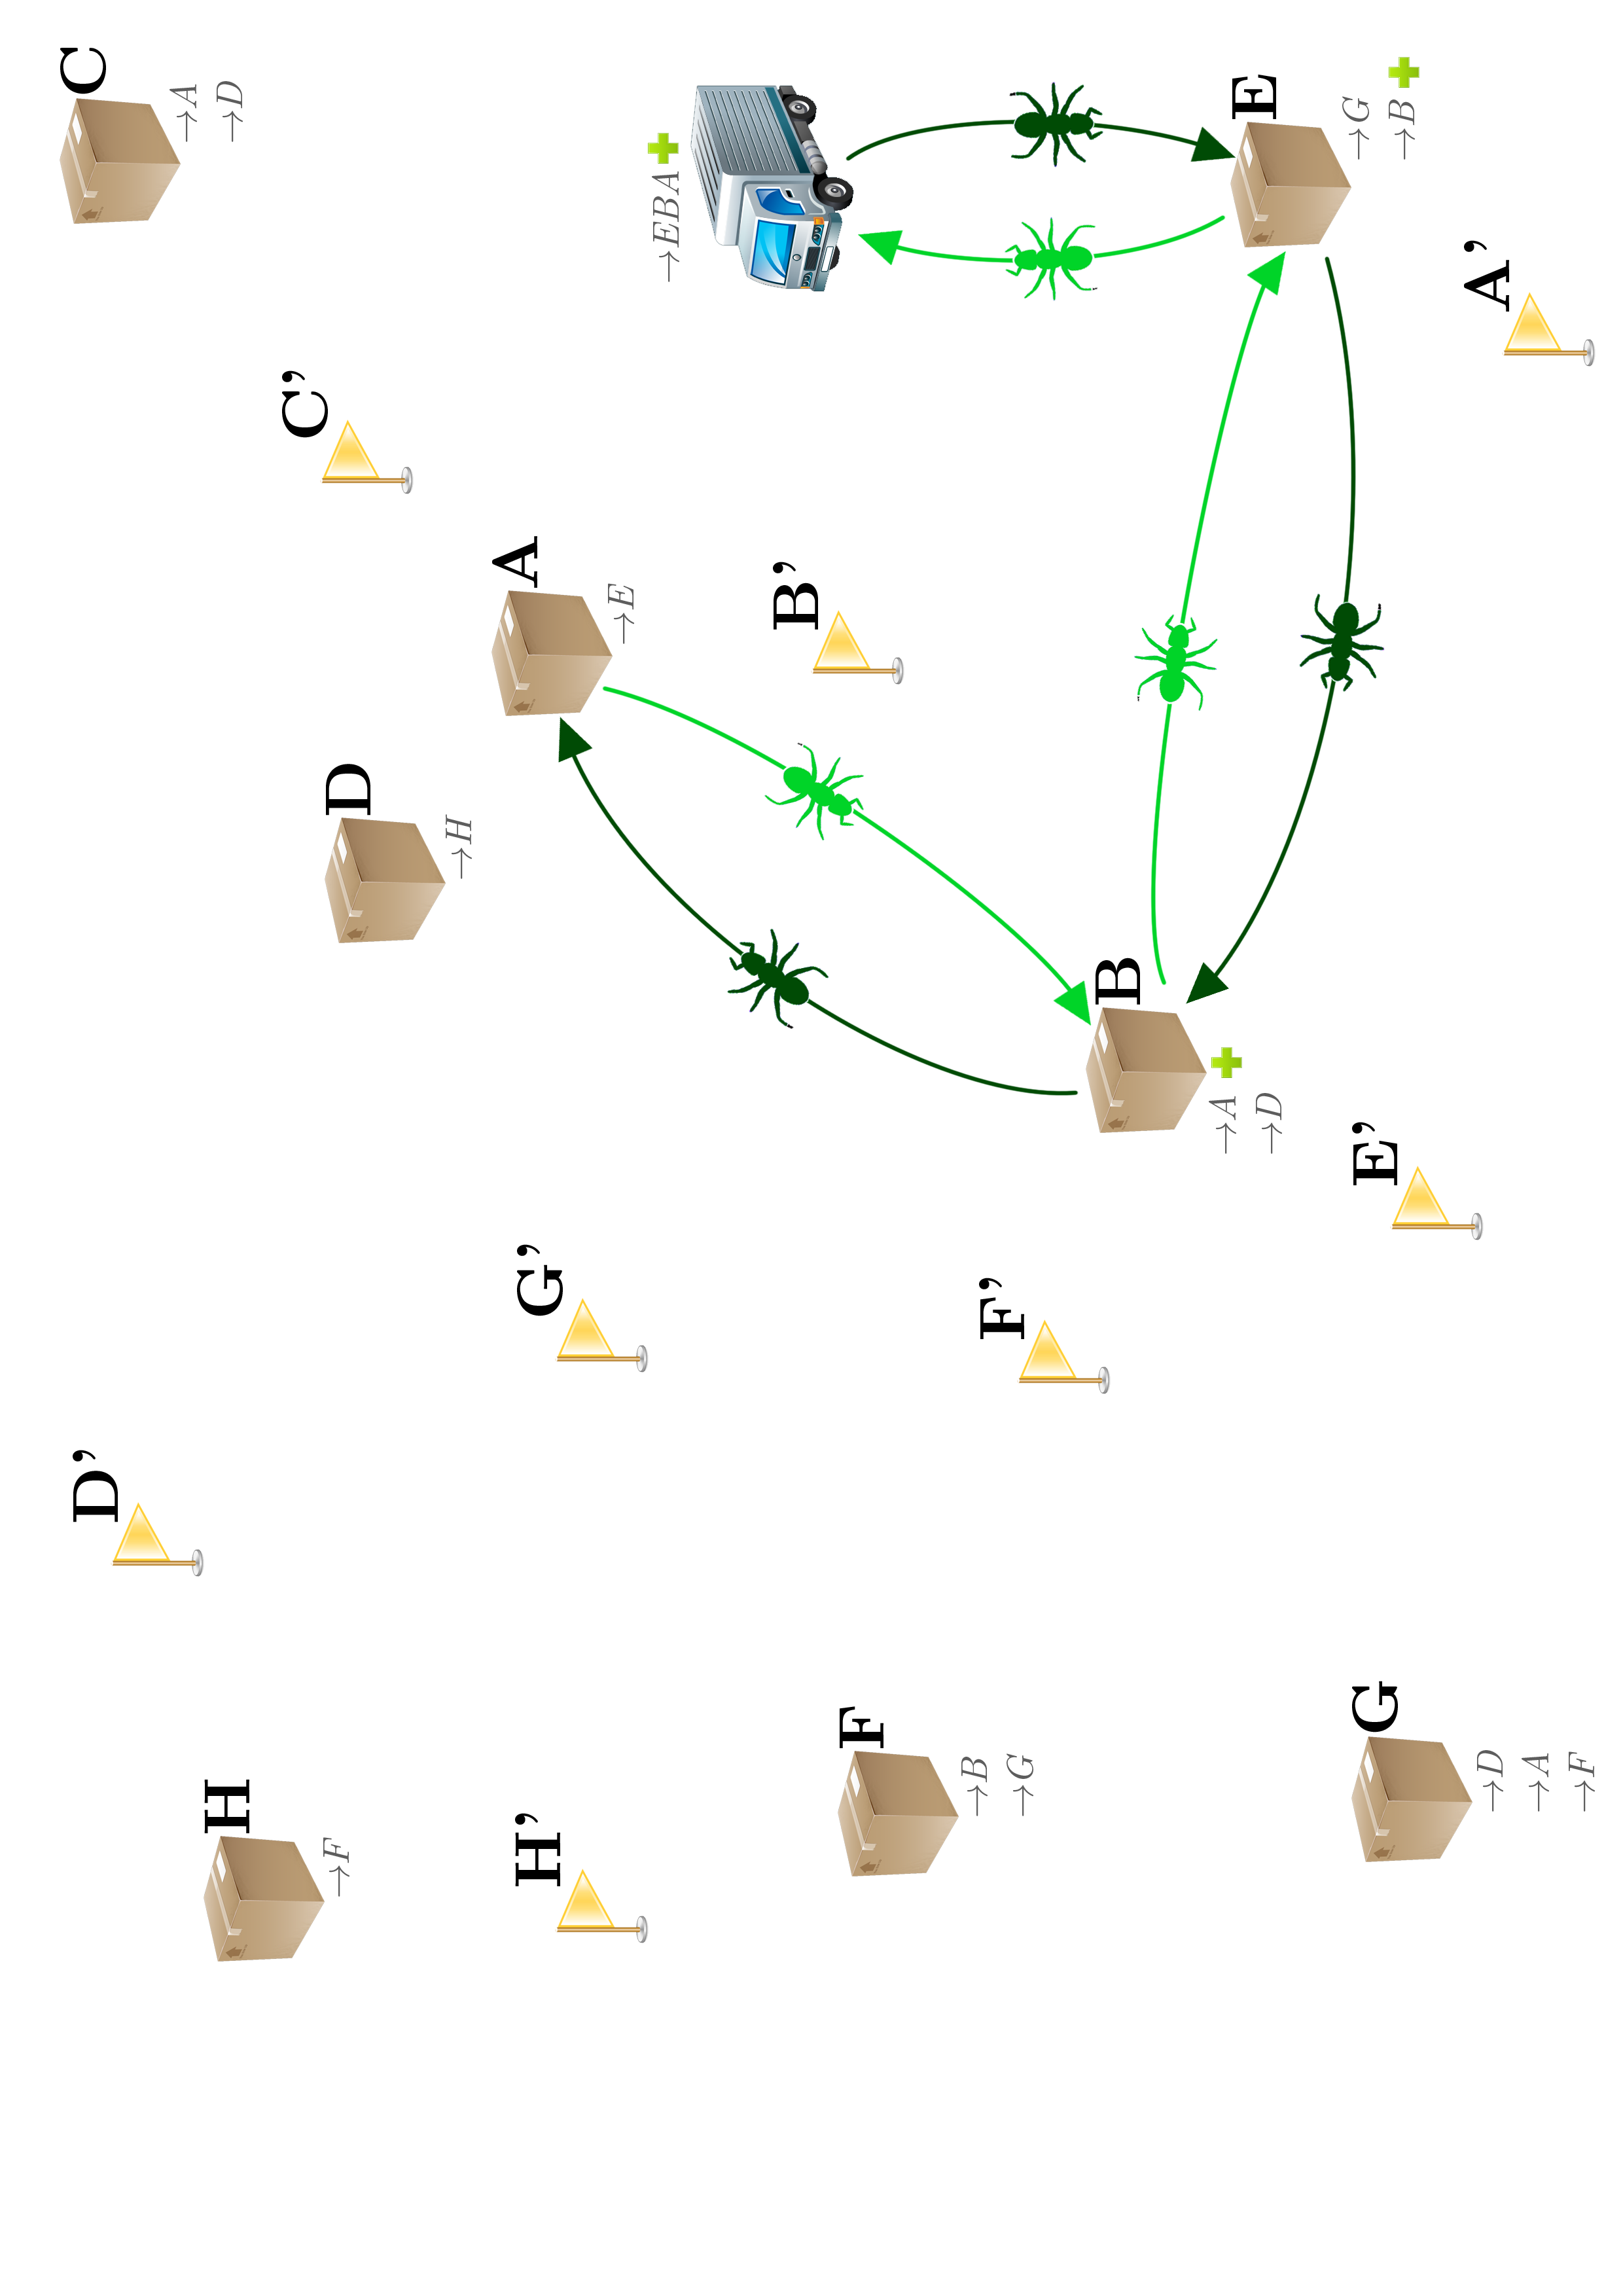
\includegraphics[width =
                0.9\textwidth]{./figs/exploration.png}}
		\end{center}
		\caption{Exploration Ants (example scenario 2)}
		\label{Fig:Radios}
        \vspace{0.5pt}
\end{figure}

\begin{figure}[!h]
        \vspace{0.5pt}
        \begin{center}
       			\setlength\fboxsep{0.5pt}
				\setlength\fboxrule{0.5pt}
                \fbox{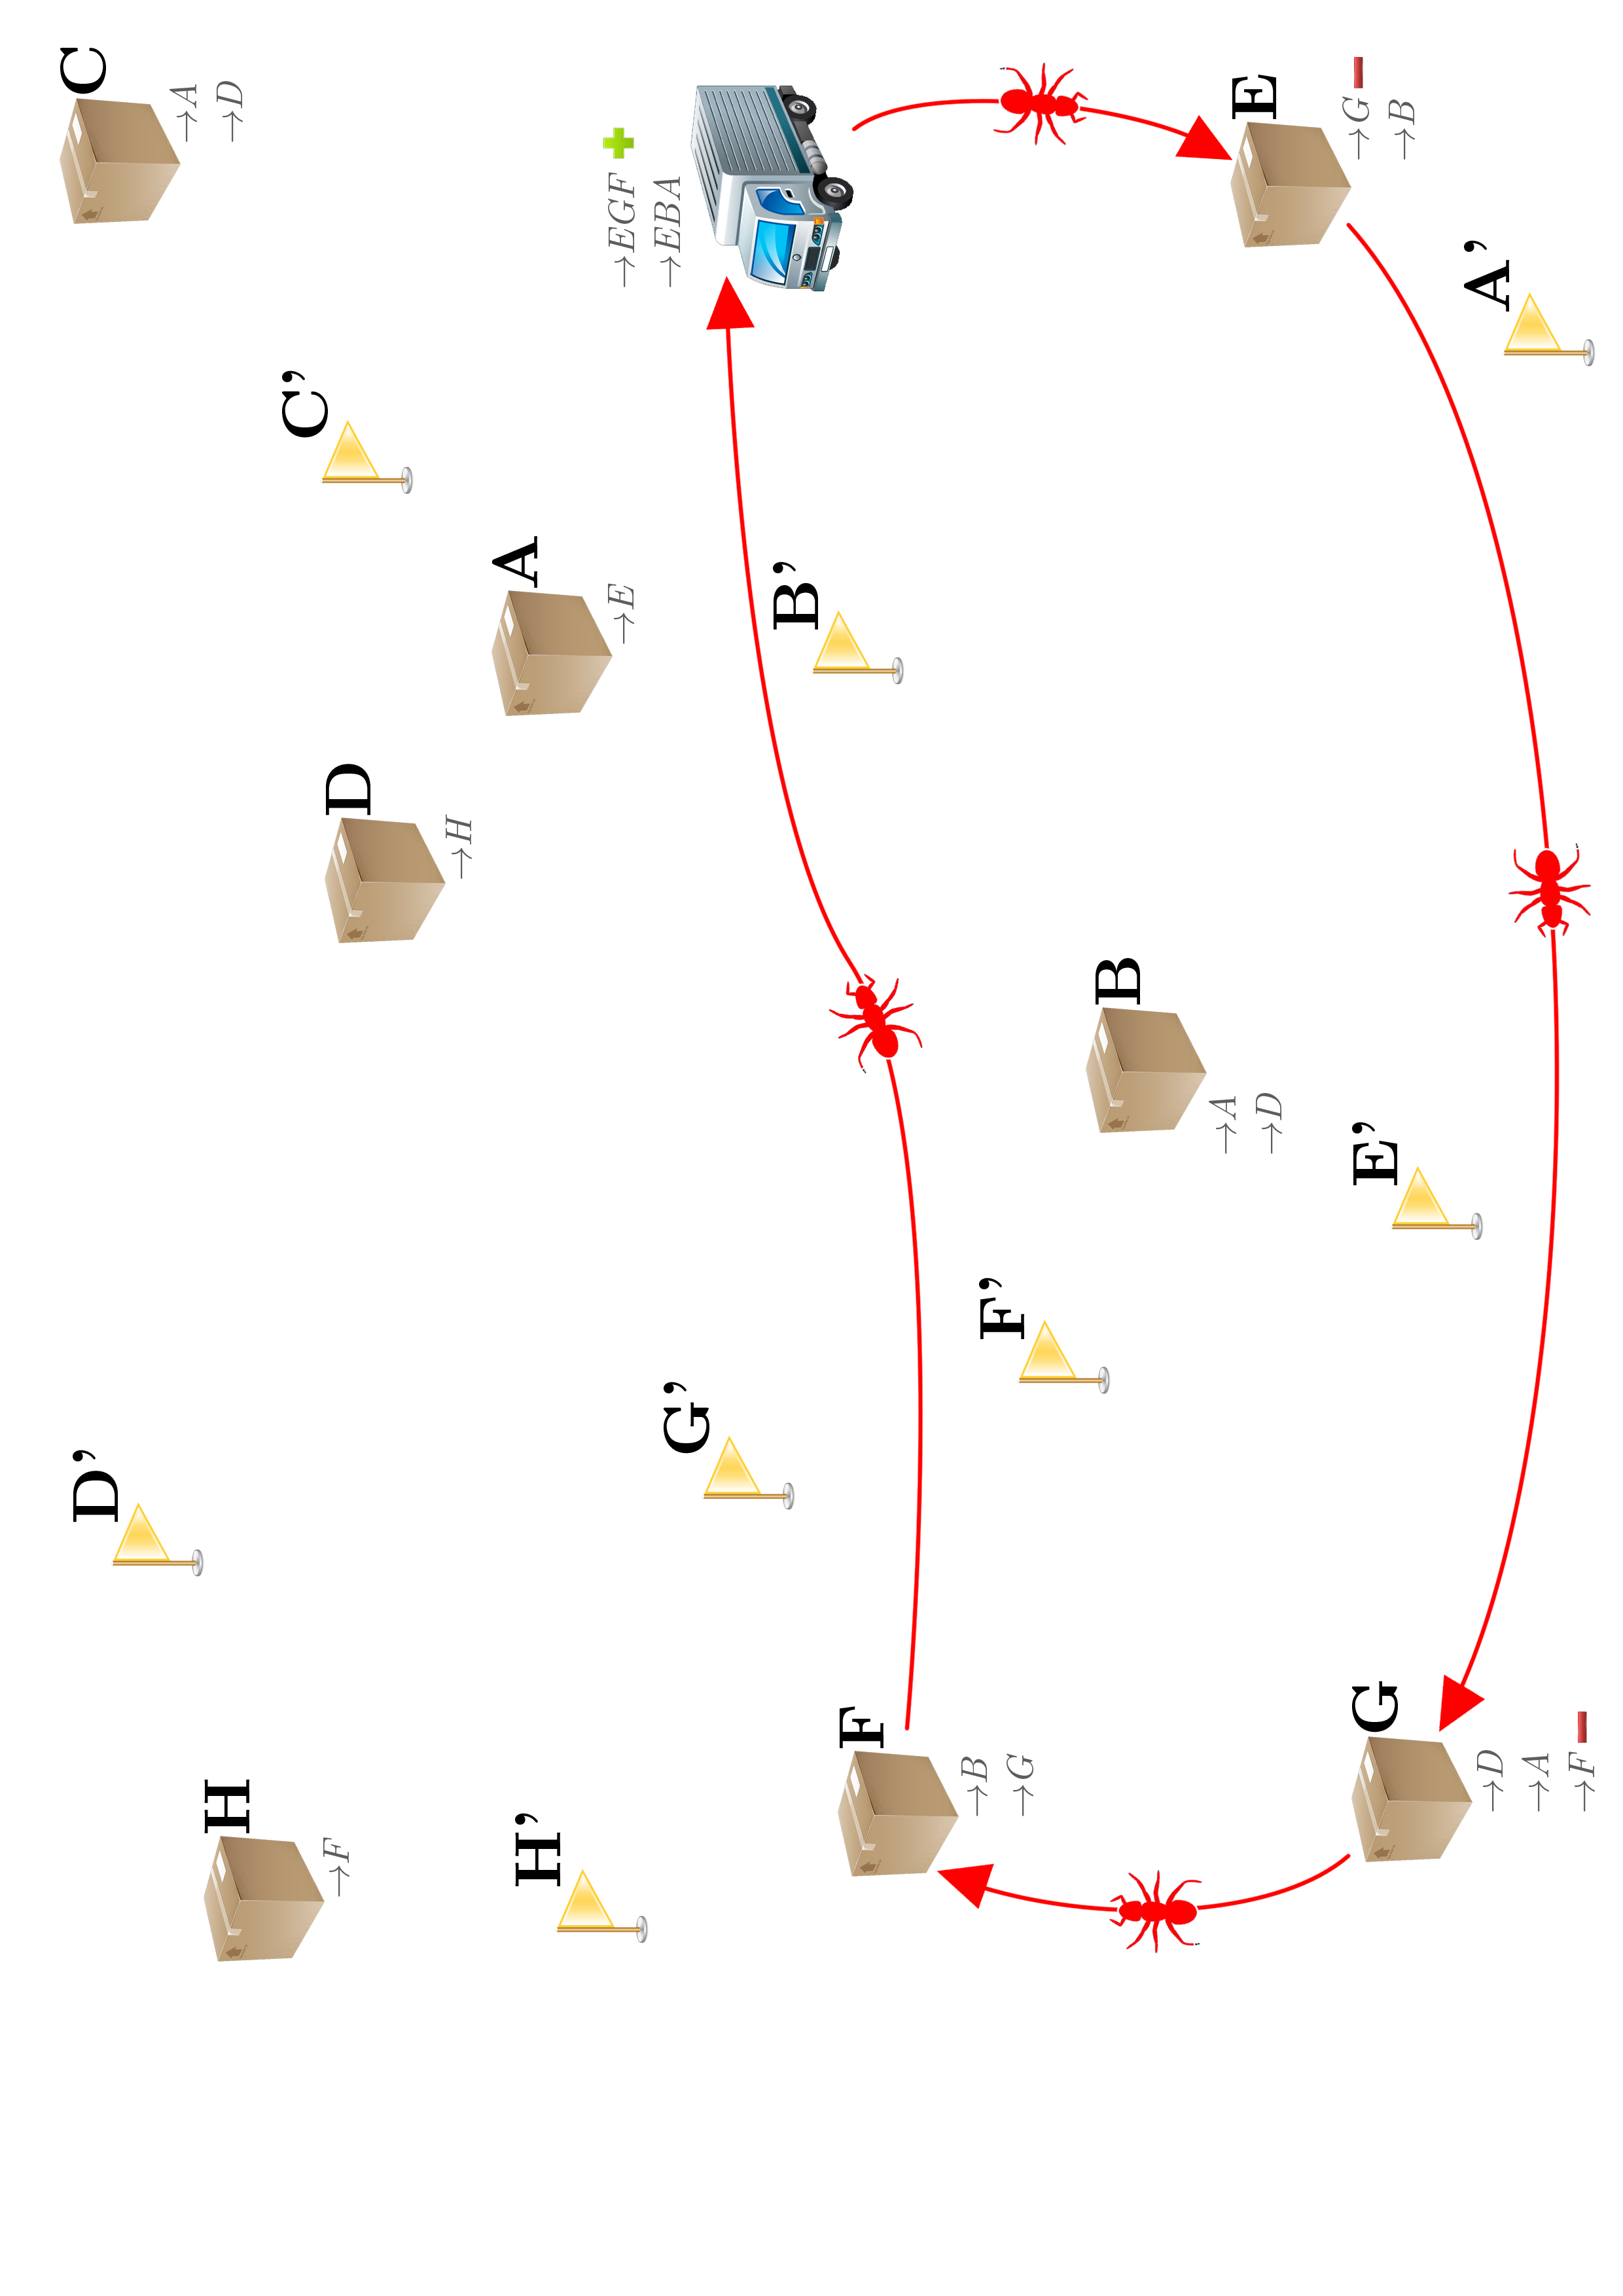
\includegraphics[width =
                0.9\textwidth]{./figs/intention.png}}
		\end{center}
		\caption{Intention Ants (example scenario 3)}
		\label{Fig:Radios}
        \vspace{0.5pt}
\end{figure}

